\documentclass[a4paper]{article}
\usepackage[affil-it]{authblk}
%\usepackage[backend=bibtex,style=numeric]{biblatex}
\usepackage{graphicx} % Required for inserting images
\usepackage{caption}

\usepackage{ctex}
\usepackage{epstopdf}
\usepackage{amsfonts,amssymb}
\usepackage{tikz}
\usetikzlibrary{chains}
\usepackage{listings}
\usepackage{xcolor}
\usepackage{float}
\usepackage{hyperref}
\usepackage{bookmark}
\usepackage{subfig}
\usepackage{listings,matlab-prettifier} % MATLAB 美化包
% \lstset{
%         style=Matlab-editor,
%         numbers      = left,
%         frame        = single,
% }
\usepackage{amsmath}
\usepackage{chngcntr}
\counterwithout{equation}{section}
\counterwithout{figure}{section}

\usepackage{geometry}
\geometry{margin=1.5cm, vmargin={0pt,1cm}}
\setlength{\topmargin}{-1cm}
\setlength{\paperheight}{29.7cm}
\setlength{\textheight}{25.3cm}


\begin{document}
% =================================================
\title{NA programming homework \#2}

\author{陈澎 Chen Peng 3220103443
  \thanks{Email: \texttt{cpzju@zju.edu.cn}}}
\affil{Xinji 2201, Zhejiang University }


\date{\today}

\maketitle

% ============================================
\section*{Problem A}


\section*{Problem B}
Complie and run the program \verb|B.cpp|. its output is the Newton interpolation polynomial of each situations.
It is shown as below.
\begin{lstlisting}[breaklines=true]
  when n=2, p(x)=0.03846+0.1923*(x+5)-0.03846*(x+5)*x
  when n=4, p(x)=0.03846+0.03979*(x+5)+0.06101*(x+5)*(x+2.5)-0.02653*(x+5)*(x+2.5)*x+0.005305*(x+5)*(x+2.5)*x*(x-2.5)
  when n=6, p(x)=0.03846+0.02646*(x+5)+0.02485*(x+5)*(x+3.333)+0.01494*(x+5)*(x+3.333)*(x+1.667)-0.01317*(x+5)*(x+3.333)*(x+1.667)*x+0.004203*(x+5)*(x+3.333)*(x+1.667)*x*(x-1.667)-0.0008406*(x+5)*(x+3.333)*(x+1.667)*x*(x-1.667)*(x-3.333)
  when n=8, p(x)=0.03846+0.02234*(x+5)+0.01396*(x+5)*(x+3.75)+0.0117*(x+5)*(x+3.75)*(x+2.5)+0.0006743*(x+5)*(x+3.75)*(x+2.5)*(x+1.25)-0.004896*(x+5)*(x+3.75)*(x+2.5)*(x+1.25)*x+0.00244*(x+5)*(x+3.75)*(x+2.5)*(x+1.25)*x*(x-1.25)-0.0006872*(x+5)*(x+3.75)*(x+2.5)*(x+1.25)*x*(x-1.25)*(x-2.5)+0.0001374*(x+5)*(x+3.75)*(x+2.5)*(x+1.25)*x*(x-1.25)*(x-2.5)*(x-3.75)
\end{lstlisting}

Use matlab to plot each p(x) and the function $\dfrac{1}{1+x^2}$ in $[-5,5]$. The image is as follows.
\begin{figure}[htbp]
  \centering
  {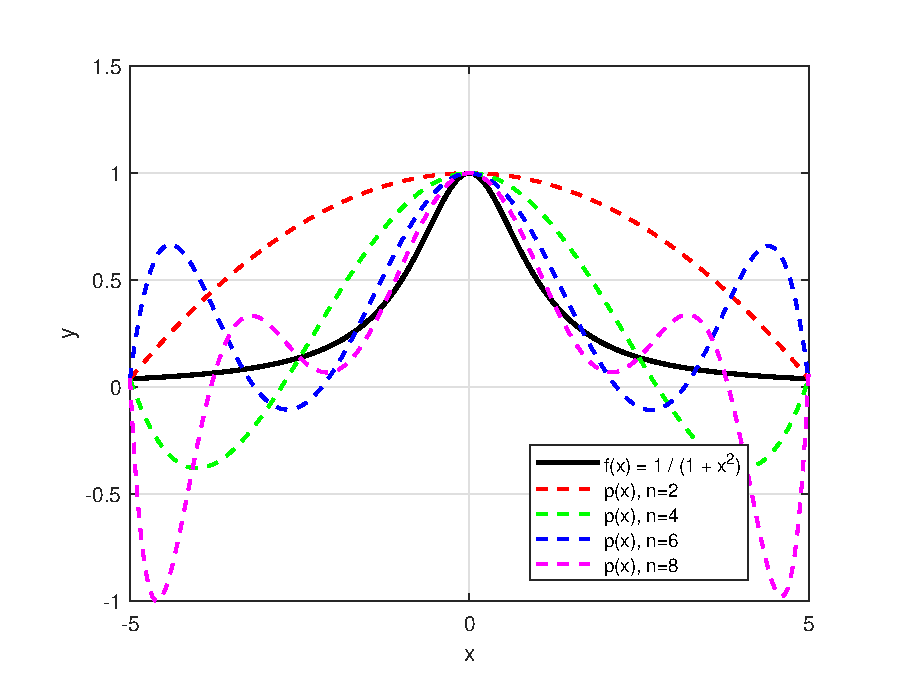
\includegraphics[width=0.6\textwidth]{images/B_pic.eps}\label{fig1}}  
  \renewcommand{\figurename}{Fig.}
  \caption{Comparison of interpolating Polynomials and Function $f(x)=\dfrac{1}{1+x^2}$}
\end{figure}

\section*{Problem C}


\section*{Problem D}


\section*{Problem E}


\section*{Problem F}

\end{document}